\documentclass[10pt, spanish]{beamer}
\usepackage[spanish]{babel}

\usetheme[progressbar=frametitle]{metropolis}

\usepackage{booktabs}
\usepackage[scale=2]{ccicons}

\usepackage{pgfplots}
\usepgfplotslibrary{dateplot}

\usepackage{float}
\graphicspath{ {images/} }

\usepackage{algpseudocode}
\usepackage{algorithm}
\usepackage{listings}

%% COLOR
\usepackage{color, colortbl}
\definecolor{Gray}{gray}{0.9}	
\definecolor{LightCyan}{rgb}{0.88,1,1}

\title{Identificaci\'on de patrones y algoritmos de consolidaci\'on en bases de datos de posicionamiento}
\date{\today}
\author{\textsc{\Large{Pilar Barbero Iriarte}}\\
Director: Tom\'as Alcal\'a Nalv\'aiz}
\institute{Universidad de Zaragoza}
\titlegraphic{\hfill
\includegraphics[height=1.5cm]{unizar.png}}

%%%%%%%%%%%%%%%%%%%%PYTHON CODING

% Default fixed font does not support bold face
\DeclareFixedFont{\ttb}{T1}{txtt}{bx}{n}{11} % for bold
\DeclareFixedFont{\ttm}{T1}{txtt}{m}{n}{11}  % for normal

% Custom colors
\usepackage{color}
\definecolor{deepblue}{rgb}{0,0,0.5}
\definecolor{deepred}{rgb}{0.6,0,0}
\definecolor{deepgreen}{rgb}{0,0.5,0}

% Python style for highlighting
\newcommand\pythonstyle{\lstset{
language=Python,
basicstyle=\ttm,
otherkeywords={self},             % Add keywords here
keywordstyle=\ttb\color{deepblue},
emph={MyClass,__init__},          % Custom highlighting
emphstyle=\ttb\color{deepred},    % Custom highlighting style
stringstyle=\color{deepgreen},
frame=tb,                         % Any extra options here
showstringspaces=false,           % 
basicstyle=\small,
columns=fullflexible,
}}


% Python environment
\lstnewenvironment{python}[1][]
{
\pythonstyle
\lstset{#1}
}
{}

% Python for external files
\newcommand\pythonexternal[2][]{{
\pythonstyle
\lstinputlisting[#1]{#2}}}

% Python for inline
\newcommand\pythoninline[1]{{\pythonstyle\lstinline!#1!}}
%%%%%%%%%%%%%%%%%%%%%%%%%%%%%%%%%

\begin{document}

\maketitle


%\section{Introducci\'on}

%%Introducci\'on
\begin{frame}[fragile]
\frametitle{Introducci\'on}
Contexto: 
\begin{itemize}
	\item Empresa Zaragozana de telecomunicaciones.
	\item Almacenamiento de posiciones GPS de sujetos.
	
	\begin{center}
		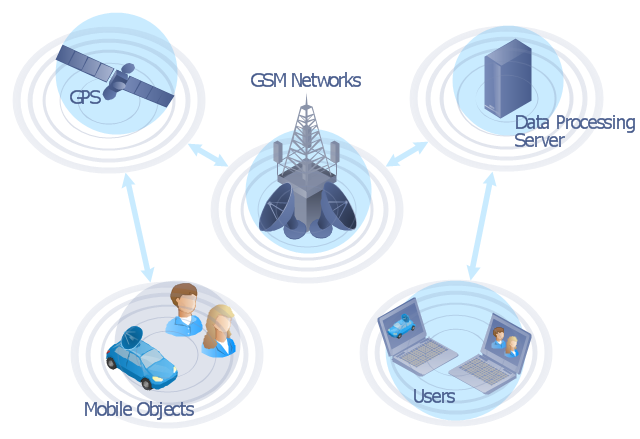
\includegraphics[scale=.45]{first.png}
	\end{center}
\end{itemize}
\end{frame}


\begin{frame}[fragile]
\frametitle{Introducci\'on}
Problemas:
	\begin{itemize}
		\item Capacidad de guardado de posiciones limitada.
		\item No existe preprocesado antes de la inserci\'on.
		\item No existe postprocesado despu\'es de la inserci\'on.
		\item No todas aportan informaci\'on.
	\end{itemize}
\end{frame}

%%OBJETIVO
\begin{frame}[fragile]
  \frametitle{Introducci\'on}
  Objetivo:
  \begin{itemize}
  	  \item Eliminar posiciones repetidas.
  	  \item Eliminar posiciones que no aporten informaci\'on.
   \end{itemize}
\end{frame}

%\section{An\'alisis de los datos}

\begin{frame}[fragile]
\frametitle{An\'alisis de los datos}
\begin{itemize}
	\item Dos bases de datos suministradas posiciones en torno a las ciudades de Salvador de Bah\'ia y R\'io de Janeiro.
	\item $1971$ recursos distintos.
	\item $4599974$ posiciones en Salvador de Bah\'ia y $6928467$ en R\'io de Janeiro.	
\end{itemize}

\begin{center}
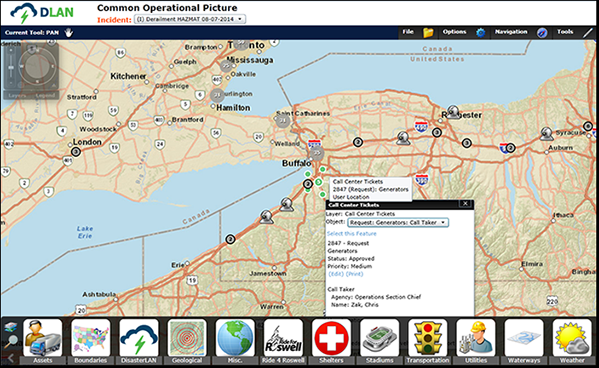
\includegraphics[scale=.55]{GIS.png}
\end{center}

\end{frame}

\begin{frame}[fragile]
\frametitle{An\'alisis de los datos}
  \begin{itemize}[<+- | alert@+>]    
\item \textbf{Id}: Identificador num\'erico
\item \textbf{IdServidor}: Identificador num\'erico del servidor que realiza la inserci\'on
\item \textbf{Recurso}: identificador del sujeto que transfiere la posici\'on
\item \textbf{Latitud}: real que representa la latitud GPS
\item \textbf{Longitud}: real que representa la longitud GPS
\item \textbf{Velocidad}: entero que representa la velocidad instant\'anea (km/h)
\item \textbf{Orientaci\'on}: entero que representa la orientaci\'on respecto al norte en grados
\item \textbf{Fecha}: dato tipo fecha que transformamos en un \texttt{timestamp}.
\item \textbf{Cobertura}: booleano que indica si tiene cobertura
\item \textbf{Error}: booleano que indica si ha habido error en la toma de posici\'on
  \end{itemize}
\end{frame}

%\section{¿C\'omo abordar el problema?}
\begin{frame}[fragile]
\frametitle{¿C\'omo abordar el problema?}
\begin{itemize}

\item Desarrollo de algoritmos de consolidaci\'on a trav\'es de nociones de distancia y tiempo.

\item Uso de algoritmos de \textit{clustering} con el fin de identificar varias posiciones con su centro del cl\'uster y consolidarlas en \'esta.

\item Se elige el el lenguaje \texttt{Python} por ser un lenguaje que tiene orientaci\'on a objetos y la gran cantidad de librer\'ias cient\'ificas de las que consta.

\end{itemize}
\end{frame}

%\section{Noci\'on de posici\'on y cl\'uster}

\begin{frame}[fragile]
\frametitle{Posici\'on}
Se define la clase \texttt{Position} en \texttt{Python} de la siguiente manera:\\
\bigskip
\begin{python}
class Position:
    def __init__(self, id, resource, lat, lon, speed, track, date):
        self.id = id
        self.resource = resource
        self.lat = lat
        self.lon = lon
        self.speed = speed
        self.track = track
        self.date = date
\end{python}
\end{frame}

%\section{M\'etodos simples}

\begin{frame}[fragile]
\frametitle{Nociones de vecindario}

Distintas nociones de vecindario para los algoritmos de consolidaci\'on simple,
\begin{itemize}
	\item Vecindad involucrando el tiempo
	\item Vecindario utilizando la distancia eucl\'idea
	\item Vecindario involucrando velocidad
	\item Vecindad $t_0-$alcanzable
\end{itemize}
\end{frame}


\begin{frame}[fragile]
\frametitle{Vecindad involucrando el tiempo}
Las posiciones de nuestros sujetos vienen muestreadas adem\'as con el instante en el que fueron tomadas.\\ \bigskip
Definimos esta distancia temporal tal que:

$$ d_T(p_0, p) = |time_p - time_{p_0}| < \delta $$

\bigskip

\begin{python}
    def is_neighboorhoudByTime(self, p, lapse):
        return abs(self.time - p.time ) < lapse
\end{python}

\end{frame}


%%%%%%%%%%%%%%%%%%%%%%%%%%%%%%
\begin{frame}[fragile]
\frametitle{Vecindario utilizando la distancia eucl\'idea}

Utilizando la distancia eucl\'idea, definimos un vecindario de la siguiente manera:\\

$$ d_E(p_0, p) = \sqrt{(lat_{p} - lat_{p_0})^2 + (long_{p} - long_{p_0})^2 } < \varepsilon $$

donde $p$ es un punto con latitud $lat_{p}$ y longitud $long_{p}$.\\

\bigskip
\begin{python}
    def IsInNeighEUSimple(self, p, eps):
        return self.distance_eu(p) < eps
\end{python}

\end{frame}

%%%%%%%%%%%%%%%%%%%%%%%%%%%%%%

\begin{frame}[fragile]
\frametitle{Vecindario involucrando velocidad}

A mayor velocidad, puntos m\'as alejados de lo que considerar\'iamos en el primer caso (fuera de nuestro vecindario simple), podr\'ian estar dentro de nuestro nuevo radio, que depender\'ia de la velocidad instant\'anea.

$$ d_E(p_0, p) = \sqrt{(lat_{p} - lat_{p_0})^2 + (long_{p} - long_{p_0})^2 } < \varepsilon \cdot vel_{p_0} $$

\bigskip
\begin{python}
    def IsInNeighSpeedRelative(self, p, eps):
        if self.speed != 0:
            return self.distance_eu(p) < eps * self.speed	
        else:
            return False
\end{python}

\end{frame}
%%%%%%%%%%%%%%%%%%%%%%%%%%%%%%
\begin{frame}[fragile]
\frametitle{Vecindad $t_0-$alcanzable}

Se fija intervalo de tiempo $t_0$, con el cual se define una vecindad $t_0$-alcanzable .\\
\bigskip
Sea la velocidad instant\'anea $vel_{p_0}$

$$ d_E(p_0, p) = \sqrt{(lat_{p} - lat_{p_0})^2 + (long_{p} - long_{p_0})^2 } < vel_{p_0} \cdot t_0 $$

\begin{itemize}
 \item A velocidad reducida, vecindad $t_0-$alcanzable menor.
 \item A mayor velocidad, mayor vecindad $t_0-$alcanzable.
\end{itemize}

\bigskip
\begin{python}
    def IsInNeighT0Reachable(self, p, t0):
        return self.distance_eu(p) < t0 * self.speed
\end{python}

\end{frame}
%%%%%%%%%%%%%%%%%%%%%%%%%%%%%%



\begin{frame}[fragile]
\frametitle{Consolidaci\'on por distancia}
Utilizando los tres tipos de vecindarios que hemos definido, definimos el
siguiente m\'etodo que realizará la consolidaci\'on del tipo que le indiquemos:\\

\bigskip

\begin{algorithmic}[1]
\Function{ConsolidationByDistance}{$positions, typeOfDistance, eps, t0$}
\For{\textbf{each} pos \textbf{in} positions}
        \If{$pos.IsInNeighBorhood(typeOfDistance, next(pos), eps)$}
        		\State{Remove pos from DB}
        \Else
        		\State{Maintain pos in DB}
        \EndIf
\EndFor
\EndFunction
\end{algorithmic}
\end{frame}


\begin{frame}[fragile]
\frametitle{Experimento utilizando consolidaci\'on por distancia}
Se fija un $\varepsilon = 0.0001$ y se realiza una consolidaci\'on utilizando la distancia eucl\'idea:\\

\bigskip

\begin{center}
	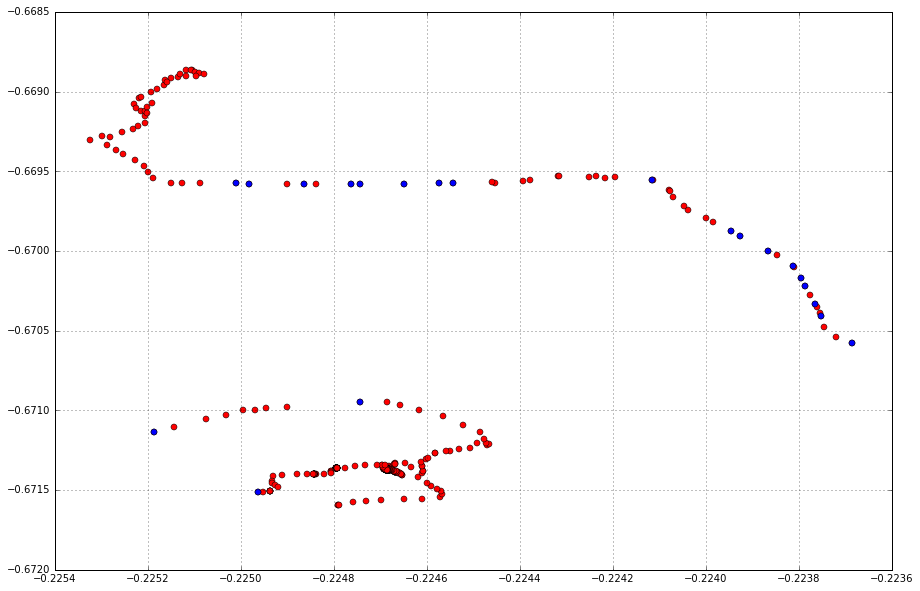
\includegraphics[scale=.3]{distanceEuEps10-4.png}¡
\end{center}

\end{frame}

\begin{frame}[fragile]
\frametitle{Consolidaci\'on por tiempo}

Se fija un lapso de tiempo que se debe cumplir entre posici\'on y posici\'on, y se eliminan todas aquellas que est\'en cuya distancia temporal con su siguiente est\'e por debajo de este lapso fijado.\\

\bigskip
\begin{algorithmic}[1]
\Function{ConsolidationByTime}{$positions, lapse$}
	\For{\textbf{each} pos in positions}
		\State{$nextpos = pos++$}
		\If{$IsInNeighboorhodByTime(nextpos, pos, lapse)$}
			\State{Remove pos}
		\EndIf
	\EndFor
\EndFunction
\end{algorithmic}
\end{frame}


\begin{frame}[fragile]
\frametitle{Experimento utilizando consolidaci\'on por tiempo}
Se realiza una consolidaci\'on por tiempo con un lapso de 20 segundos:\\

\bigskip

\begin{center}
	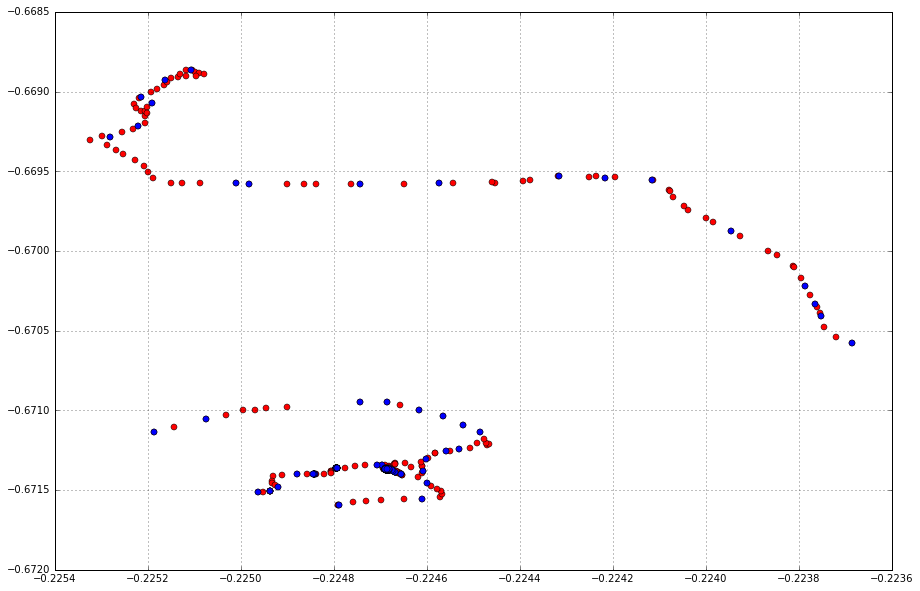
\includegraphics[scale=.3]{byTimeSuj1.png}
\end{center}

\end{frame}


\begin{frame}[fragile]
\frametitle{Consolidaci\'on por adelgazamiento}
Se puede recurrir a un tipo de consolidaci\'on en la cual dada una lista de posiciones normalmente antiguas, se elimine un subconjunto de estas, por ejemplo, 3 de cada 5.\\
\bigskip
\begin{algorithmic}[1]
\Function{ConsolidationByThinning}{$positions, j, k$}\Comment{$j < k$}
	\For{\textbf{each} pos in positions}
		\If{$position.Index \% k == 0$}
			\For{$i = 0; i < j; i++$}
				\State{Remove position with index == position.Index}
			\EndFor
		\EndIf
	\EndFor
\EndFunction
\end{algorithmic}
\end{frame}


\begin{frame}[fragile]
\frametitle{Experimento utilizando consolidaci\'on por adelgazamiento}
Se realiza una consolidaci\'on por adelgazamiento, se mantienen 2 posiciones de cada 5:\\

\bigskip

\begin{center}
	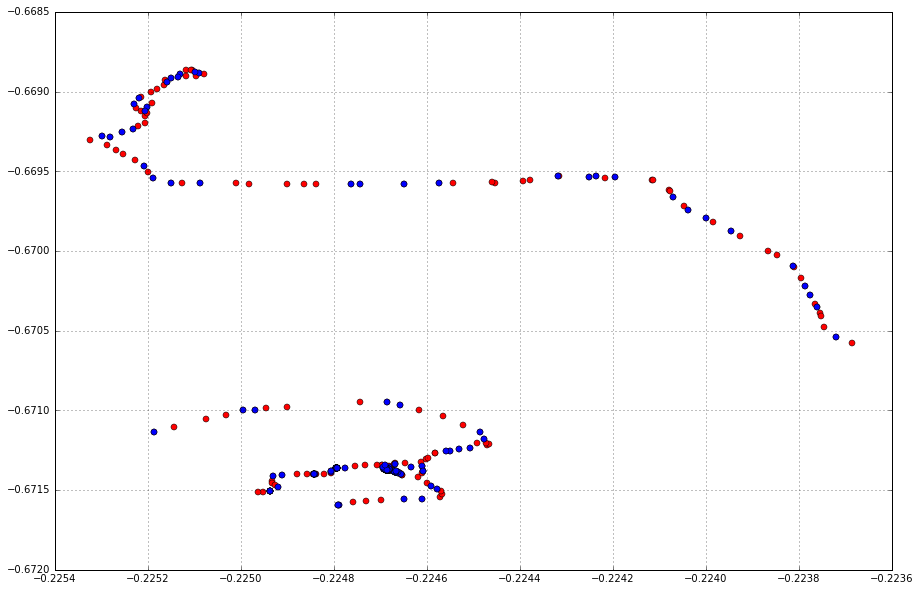
\includegraphics[scale=.3]{thinningSuj1.png}
\end{center}

\end{frame}



\begin{frame}[fragile]
\frametitle{M\'etodos avanzados}

\textbf{Algoritmos de consolidaci\'on asociados a m\'etodos de clustering}\\

\begin{itemize}
   \item T\'ecnica o conjunto de t\'ecnicas multivariantes utilizadas en Miner\'ia de datos y Modelizaci\'on matem\'atica utilizadas para clasificar a un conjunto de individuos en grupos homog\'eneos.
\end{itemize}

\textbf{Algoritmos a analizar}:\\
\begin{itemize}
\item \textbf{K-means}
\item \textbf{DBSCAN}
\item \textbf{DJ-Cl\'uster}
\end{itemize}

\end{frame}


\begin{frame}[fragile]
\frametitle{K-means}
\textbf{K-means} es un m\'etodo eficiente de \textit{clustering} que tiene como objetivo la partici\'on de un conjunto de $n$ elementos en $k$ grupos distintos. Dado un conjunto de $n$ elementos, se construye dicha partici\'on $S=\{S_1, S_2, \ldots, S_k\}$ con el fin de minimizar el t\'ermino del error cuadr\'atico:

$$ \sum_{i=1}^{n} \sum_{x\in S_i} \text{d}(x,m_i)$$

donde $m_i$ es el centro de cada cl\'uster $S_i$ y $\text{d}(x, m_i)$ es la distancia definida entre el punto $x$ y $m_i$.

\end{frame}

\begin{frame}[fragile]
\frametitle{K-means}
Se procede:
\begin{enumerate}
	\item Se prefija un n\'umero de cl\'usters.
	\item Conformamos los primeros centroides de los grupos de manera aleatoria.
	\item Se itera sobre cada punto, encuentra el centro de cl\'uster m\'as cercano y se lo asigna a dicho cl\'uster.
	\item Se recalcula los centroides de los cl\'usters y se reitera hasta que el error cuadr\'atico se minimiza o se estabiliza.
\end{enumerate}
\end{frame}

\begin{frame}[fragile]
\frametitle{Experimento con K-means}
Se utiliza el software \texttt{Weka} sobre un sujeto con $2000$ posiciones para una consolidaci\'on al $25\%$, es decir, a $500$.

\begin{center}
	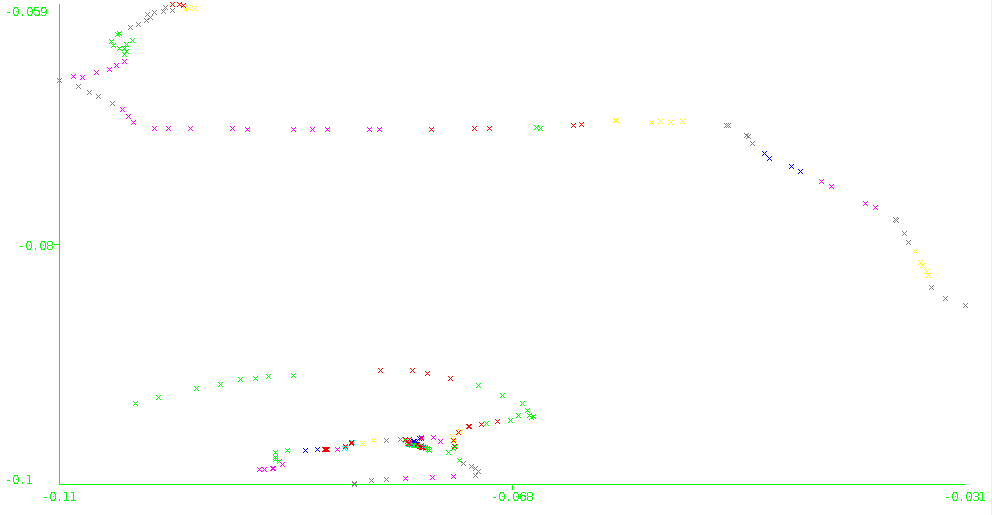
\includegraphics[scale=.43]{kMeansSujeto1.png}
\end{center}


\end{frame}

\begin{frame}[fragile]
\frametitle{Conclusiones K-means}

Resultados:
\begin{itemize}
\item 10 iteraciones 
\item Error cuadr\'atico: 0,117363
\item n\'umero de posiciones que ha agrupado por cl\'uster entre 1 y 9
\end{itemize}

\bigskip

Inconvenientes:
\begin{itemize}
	\item N\'umero de cl\'usters prefijado a 500.
	\item K-means no determin\'istico.
	\item No hay puntos considerados ruidos, s\'olo cl\'usters unipuntuales.
\end{itemize}
\end{frame}


%%%%%%%%%%%%%%%%%%%%%%%%%%%%%%%%%%%%%%%%%
%%%%%%%%%%%%%%%%%%%%%%%%%%%%%%%%%%%%%%%%%\\
%%%%%%%%%%%%%%%%%%%%%%%%%%%%%%%%%%%%%%%%%

\begin{frame}[fragile]
\frametitle{DBSCAN}
\textbf{DBSCAN}  es un algoritmo de clustering basado en la densidad por lo que encuentra el n\'umero de cl\'usters comenzando por una estimación de la distribución
de densidad de los nodos correspondientes. \\

\begin{itemize}
\item Punto $p$ n\'ucleo: si posee un n\'umero m\'inimo de puntos ($minPts$) en su vecindario sobre $\varepsilon$.
\item Punto $q$ alcanzable por $p$: si existe un camino $p_1, \ldots, p_n$ tal que $p_i$ est\'a en el vecindario de $p_{i+1}$ (o viceversa).
\item Aislados: puntos no considerados ni n\'ucleo ni alcanzables.

\end{itemize}
\smallskip
\begin{center}

	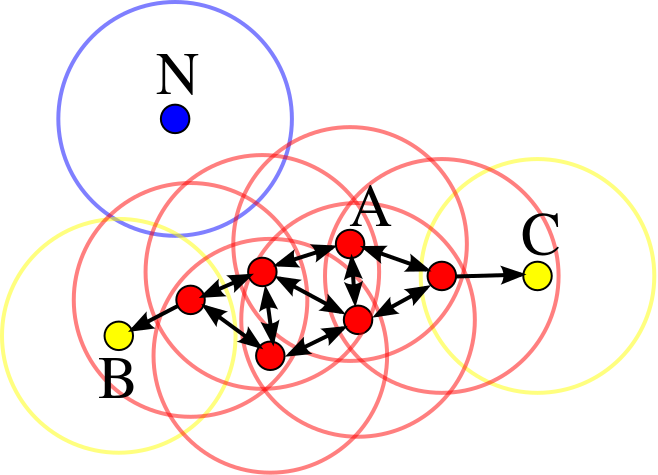
\includegraphics[scale=.25]{DBSCAN.png}
	
\end{center}
\end{frame}

\begin{frame}[fragile]
\frametitle{DBSCAN}
\textbf{DBSCAN} necesita de dos par\'ametros: $\varepsilon$ y $MinPts$.

\begin{algorithmic}[1]
\Function{DBSCAN}{$positions, eps, minPts$}
	\State{C = 0}
	\For{\textbf{each} pos in positions}
		\If{$pos$ has been visited}
			\State{Continue next position}
		\Else
			\State{Mark $pos$ as visited}
			\State{N(pos) = NeighborPts(pos, eps)}
			\If{$length(N(pos)) < MinPts$}
				\State{Mark $pos$ as noise}
			\Else
				\State{C = next Cluster}
				\State{expandCluster(pos, N(pos), C, eps, MinPts)}				
			\EndIf
		
		\EndIf
	\EndFor
\EndFunction
\end{algorithmic}
\end{frame}

\begin{frame}[fragile]
\frametitle{Experimento con DBSCAN}
Elegimos un $\varepsilon = 0.0001$ y $minPts = 5$ ya que nos proporcionar\'ia una consolidaci\'on de aprox. $20\%$.\\
\begin{center}
	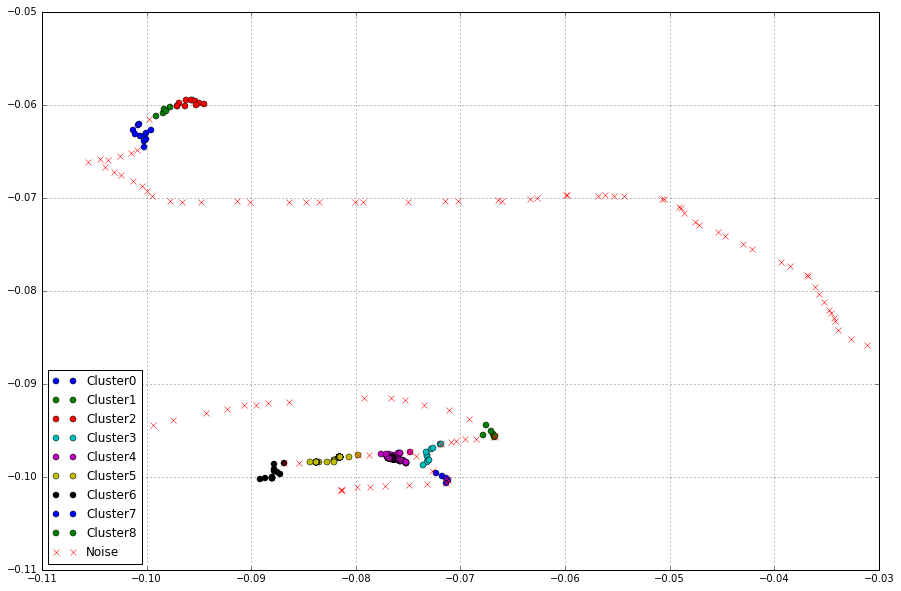
\includegraphics[scale=.3]{dbscanSujeto1.png}
\end{center}
\end{frame}

\begin{frame}[fragile]
\frametitle{Experimento con DBSCAN}
Resultados:\\
\begin{itemize}
\item 9 cl\'usters
\item Muchos puntos marcados como ruido
\end{itemize}

Inconvenientes:
\begin{itemize}
\item Decididir si esos puntos marcados como ruido son eliminables o no.
\end{itemize}
\end{frame}

%%%%%%%%%%%%%%%%%%%%%%%%%%%%%%%%%%%%%%%%%%%%%%%%%
%%%%%%%%%%%%%%%%%%%%%%%%%%%%%%%%%%%%%%%%%%%%%%%%%\\
%%%%%%%%%%%%%%%%%%%%%%%%%%%%%%%%%%%%%%%%%%%%%%%%%
%%%%%%%%%%%%%%%%%%%%%%%%%%%%%%%%%%%%%%%%%%%%%%%%%\\
%%%%%%%%%%%%%%%%%%%%%%%%%%%%%%%%%%%%%%%%%%%%%%%%%

\begin{frame}[fragile]
\frametitle{DJ-Cluster}
\textbf{Density-Joinable Cl\'uster} es un tipo de algoritmo de clustering basado en densidades de puntos. \\

\begin{enumerate}
	\item Para cada punto, calculamos su vecindario fijado un $\varepsilon$.
	\item Si el n\'umero de puntos del vecindario es menor que $minPts$, se deshecha.
	\item Si el n\'umero de puntos es mayor que $minPts$, se crea un cl\'uster.
	\item Se comprueba si existen cl\'usters densamente acoplables (si existen otros cl\'usters con alg\'un punto en com\'un)
\end{enumerate}

\begin{center}
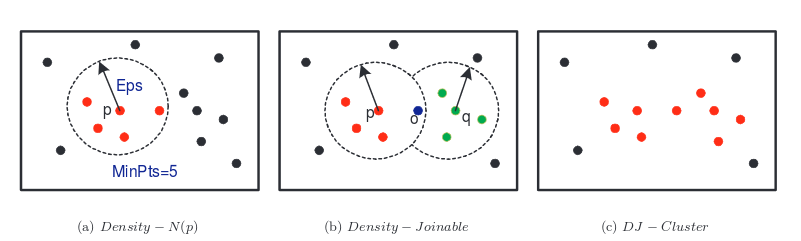
\includegraphics[scale=.45]{djcluster.png}
\end{center}
\end{frame}

\begin{frame}[fragile]
\frametitle{DJ-Cluster}
\begin{algorithmic}[1]
	\For{\textbf{each} $p$ in set $S$}
		\State{Compute neighborhood $N(p)$ for $\varepsilon$ and $MinPts$}
		\If{$N(p)$ is null ($|N(p)| < MinPts$ for $\varepsilon$)}
			\State{Label $p$ as noise}
		\ElsIf{$N(p)$ is density-joinable to an existing cluster} 
			\State{Merge $N(p)$ with the cluster which is density-joinable}
		\Else
			\State{Create a new cluster $C$ based on $N(p)$}
		\EndIf
	\EndFor
\end{algorithmic}

\end{frame}

\begin{frame}[fragile]
\frametitle{Experimento con DJ-Cluster}
Utilizando \texttt{Weka} dado un $\varepsilon=0.0001$ y $minPts = 2$:\\

\begin{center}
	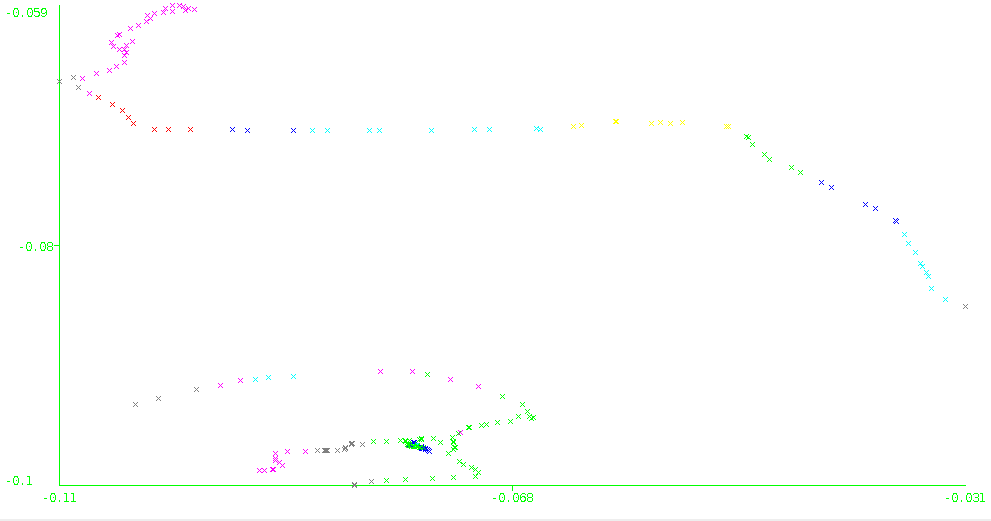
\includegraphics[scale=.43]{djClusterSujeto1.png}
\end{center}

\end{frame}

\begin{frame}[fragile]
\frametitle{Experimento con DJ-Cluster}

\centering
22 cl\'usters en total:\\

\bigskip
\begin{tabular}{|r|r|}
\hline
\rowcolor{Gray}
N. Cl\'uster & Cantidad puntos \\
\hline
0 & 3 \\ 
12 & 605\\
58 & 7\\
142 & 449\\
.... & ... \\
\hline
\end{tabular}

\end{frame}



%%%%%%%%%%%%%%%%%%%%%%%%%%%%%%%%%%%%%%%%%%%%%%%%%
%%%%%%%%%%%%%%%%%%%%%%%%%%%%%%%%%%%%%%%%%%%%%%%%%\\
%%%%%%%%%%%%%%%%%%%%%%%%%%%%%%%%%%%%%%%%%%%%%%%%%
%%%%%%%%%%%%%%%%%%%%%%%%%%%%%%%%%%%%%%%%%%%%%%%%%\\
%%%%%%%%%%%%%%%%%%%%%%%%%%%%%%%%%%%%%%%%%%%%%%%%%

\begin{frame}[fragile]
\frametitle{Comparativa t\'ecnicas simples}

Se ha realizado estos experimentos sobre el mismo sujeto tomando una muestra de las primeras $2000$ posiciones en el tiempo.\\

\begin{center}
\begin{tabular}{|l|l|l|}
	\hline
	\rowcolor{Gray}
	M\'etodo & Tiempo & N. \\
	\hline	
	Cons. por adelgazamiento &  <0.01 sec & 800 \\
	\hline 
	Cons. por distancia simple &  <0.01 sec & 507 \\
	\hline
	Cons. por distancia $t_0-$alcanzable  &  <0.01 sec  & 21\\
	\hline
	Cons. por tiempo &  <0.01 sec  & 1786\\
	\hline
\end{tabular}
\end{center}

\end{frame}

%\section{Comparativa casos estudiados}
\begin{frame}[fragile]
\frametitle{Comparativa t\'ecnicas clustering}
\begin{center}
\begin{tabular}{|l|l|l|l|}
	\hline
	\rowcolor{Gray}
	M\'etodo & Tiempo & Cl\'usters & Iteraciones\\
	\hline	
	K-means & 0.69 secs & 500 & 9\\
	\hline
	DBSCAN &  2 min 30 secs & 9 & 111 \\
	\hline
	DJ-Cluster &  0.37 secs & 22  & 11\\
	\hline
\end{tabular}
\end{center}

\begin{itemize}
	\item DBSCAN m\'as lento de todos.
	\item DBSCAN consolidaci\'on mayor.
	\item K-means se queda en 500 cl\'usters.
	\item DJ-Cl\'uster baja de los 500.
	\item DJ-Cl\'uster menor tiempo de ejecuci\'on.
\end{itemize}

\end{frame}



%\section{Conclusiones}
\begin{frame}[fragile]
\frametitle{Conclusiones}
\textbf{Algoritmos de consolidaci\'on simple:}
\begin{enumerate}[<+- | alert@+>]
	\item Son \textit{simples}, pero eficaces.
	\item Noci\'on de vecindario distinto al eucl\'ideo implementada en algoritmos de consolidaci\'on simple.
\end{enumerate}

\textbf{Algoritmos de clustering:}
\begin{enumerate}[<+- | alert@+>]
	\item M\'as avanzados, pero m\'as complejos a la hora de implementar.
	\item Importante un procesado previo.
	\item Mejores a la hora de recuperar una traza con los datos borrados.
	\item Nociones de ruido implementadas.
\end{enumerate}
\end{frame}

%\section{Demostraci\'on}

\begin{frame}[fragile]
\frametitle{Demostraci\'on}
\texttt{IPython Notebook}
\end{frame}

\begin{frame}[fragile]
	\frametitle{C\'odigo}
	\begin{center}
		\href{http://github.com/pbarbero/TFM}{http://github.com/pbarbero/TFM}
		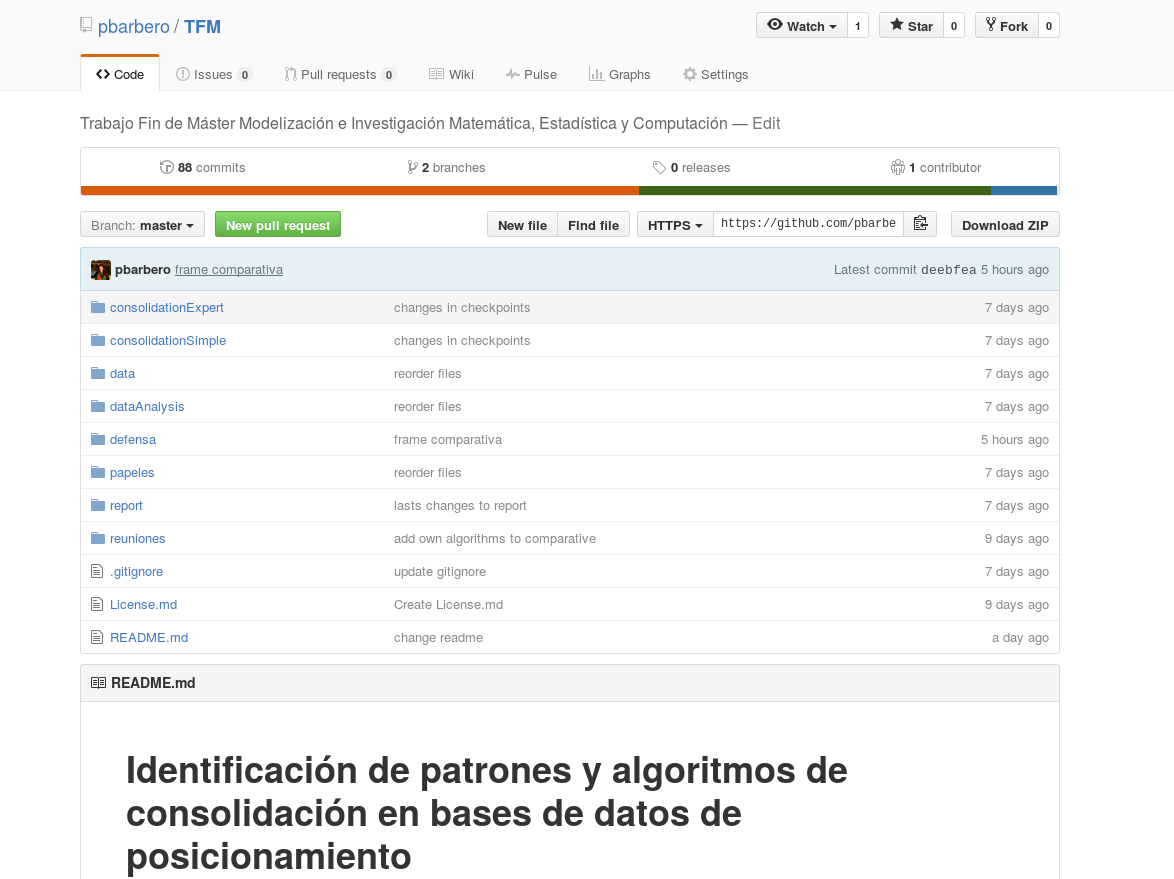
\includegraphics[scale=.3]{github.png}
	\end{center}
\end{frame}

\begin{frame}[fragile]
\frametitle{Referencias}
\begin{itemize}
\item \textsc{Frank E. and Witten I.H.} Data Mining: Practical Machine Learning Tools and Techniques. Morgan Kaufmann, San Francisco, 2nd edition, 2005.

\item \textsc{Terveen L. Frankowski D., Ludford P. Shekhar S. and Zhou C.} Discovering personal gazetteers: An interactive clustering approach. In In Proc. ACMGIS, pages 266–273. ACM Press, 2004.

\item \textsc{Nigam K. McCallum A. and Ungar L. H.} Efficient clustering of high dimensional data sets with application to reference matching, 2000.

\item \textsc{Kafle S.} Implementation of dbscan algorithm in python. \href{https://github.com/SushantKafle/DBSCAN, 2014.}{https://github.com/SushantKafle/DBSCAN}, 2014.


\end{itemize}

\end{frame}

%\section{Preguntas}



\end{document}
